\lecture{5}{02.05.2017}{Dr. Raphael Kruse}{Frank Rehfeld}
\begin{definition}
	$\left(X,\|\cdot\|_{X}\right),\left(Y,\|\cdot\|_{Y}\right)$ seien Banachräume. Eine lineare, injektive Abbildung
	\begin{equation*}
		j\colon X\to Y
	\end{equation*}
	wird \textbf{Einbettung} genannt. $X$ kann also mit $j\left(X\right)$ identifiziert werden.
	\begin{itemize}
		\item Ist $j$ stetig, so sagt man, $X$ ist stetig in $Y$ eingebettet ($X\hookrightarrow Y$).
		\item Ist $j$ kompakt, so sagt man, $X$ ist kompakt in $Y$ eingebettet ($X\cembed Y$)
		\item Ist $j\left(X\right)$ dicht in $Y$ und $X\hookrightarrow Y$, so sagt man, $X$ ist dicht in $Y$ eingebettet ($X\dembed Y$)
	\end{itemize}
\end{definition}

\begin{lemma}[Satz]
	$u\in\H^{1}\left(\W\right)$ ist fast überall gleich einer absolut stetigen Funktion.\\
	$\H^{1}\left(\W\right)\cembed\C\left(\overbar{\W}\right)$
\end{lemma}
\begin{proof}
	Mithilfe der Cauchy-Schwarz-Ungleichung erhalten wir $\L^{2}\left(\W\right)\hookrightarrow\L^{1}\left(\W\right)$ und somit $\H^{1}\left(\W\right)\hookrightarrow W^{1,1}\left(\W\right)$ und somit die erste Aussage.
	
	Sei $u\in\H^{1}\left(\W\right)${}
	\begin{align*}
		\|u\|_{\infty} &\leq \frac{\operatorname{max}\left(1,b-a\right)}{b-a}\left(\int_{a}^{b}|u\left(\xi\right)|\d\xi + \int_{a}^{b}|u^{\prime}\left(\xi\right)\d\xi\right)\\
		&\overset{\mathclap{\text{CSU}}}{\leq} \hspace*{1em} \frac{\operatorname{max}\left(1,b-a\right)}{b-a}\left(\int_{a}^{b}1\d\xi\right)^{1/2}\left(\int_{a}^{b}\left(|u\left(\xi\right)|+|u^{\prime}\left(\xi\right)|\right)^{2}\d\xi\right)^{1/2}\\
		&\leq \sqrt{2}\frac{\operatorname{max}\left(1,b-a\right)}{b-a}\left(\int_{a}^{b}1\d\xi\right)^{1/2}\left(\int_{a}^{b}|u\left(\xi\right)|^{2}+|u^{\prime}\left(\xi\right)|^{2}\d\xi\right)^{1/2}\\
		&\leq \sqrt{2}\frac{\operatorname{max}\left(1,b-a\right)}{\sqrt{b-a}}\|u\|_{1,2}
	\end{align*}
	und somit haben wir $\H^{1}\left(\W\right)\hookrightarrow \C\left(\overbar{\W}\right)$.\\
	Sei $\left(u_{n}\right)\subset\H^{1}\left(\W\right)$ eine bezüglich $\|\cdot\|_{1,2}$ beschränkte Folge. Dann ist $\left(u_{n}\right)$ auch bezüglich $\|\cdot\|_{\infty}$ beschränkt. Mit
	\begin{align*}
		|u_{n}\left(x_{1}\right)-u_{n}\left(x_{2}\right)| &= \int_{\operatorname{min}}^{\operatorname{max}}u^{\prime}_{n}\left(\xi\right)\d\xi\\
			&< \sqrt{|x_{1}-x_{2}|}\underbrace{\left(\int_{\W}|u^{\prime}_{n}\left(\xi\right)|^{2}\d\xi\right)^{1/2}}_{\leq \|u\|_{1,2} \leq M}
	\end{align*}
	erhalten wir, dass $\left(u_{n}\right)$ gleichgradig stetig ist. Wir erhalten mit Arzela-Ascoli, dass $\left(u_{n}\right)$ kompakt ist und $\H^{1}\left(\W\right)\cembed\C\left(\overbar{\W}\right)$
\end{proof}

\begin{lemma}[Satz]
	$C^{\infty}\left(\W\right)$ liegt dicht in $H^{1}\left(\W\right)$.
\end{lemma}
\begin{lemma}
	$u\in\H^{1}\left(\W\right), 0<\e_{0}<\frac{b-a}{2}$.\\
	$\implies u_{\e} = J_{e}\star u\overset{\mathclap{\e\to 0}}{\rightarrow}u$ bezüglich $\|\cdot\|_{1,2}$ auf $\left(a-\e,b+\e\right)$.
\end{lemma}
\begin{proof}
	$x\in\left(a+\e_{0},b-\e_{0}\right), \e\in\left(0,\e_{0}\right)$. Es sei $\phi\colon y\mapsto J_{\e}\left(x-y\right)\in\C^{\infty}_{\text{c}}\left(\R\right)$. Dann gilt
	\begin{equation*}
		\operatorname{supp}\left(\phi\right) = \left[x-\e,x+\e\right]\subset\left(a,b\right)
	\end{equation*}
	und somit $\phi\in\C^{\infty}_{\text{c}}\left(\W\right)$. Es folgt also $\forall x\in\left(a+\e_{0},b-\e_{0}\right),\e\in\left(0,\e_{0}\right)${}
	\begin{align*}
		\left(u^{\prime}\right)_{\e}\left(x\right) &= \int_{\W}J_{\e}\left(x-y\right)u^{\prime}\left(y\right)\d y\\
			&= -\int_{\W}\frac{\partial}{\partial y}J_{\e}\left(x-y\right)u\left(y\right)\d y\\
			&\overset{\mathclap{\text{Kette}}}{=}\hspace*{1em}\left(-1\right)^{2}\int_{\W}J^{\prime}_{\e}\left(x-y\right)u\left(y\right)\d y\\
			&\overset{\mathclap{\text{Majorante}}}{=}\hspace*{1.5em}\frac{\partial}{\partial x}\int_{\W}J_{\e}\left(x-y\right)u\left(y\right)\d y = \left(u_{\e}\right)^{\prime}\left(x\right)
	\end{align*}
	Somit folgt $u_{\e}\to u$ und $\left(u^{\prime}\right)_{\e}\to u^{\prime}$ in $\L^{2}\left(a+\e_{0},b-\e_{0}\right)$.
\end{proof}
\begin{prf}[des Satzes]
	\begin{multicols}{2}
	\begin{enumerate}
		\item{}
			Seien $I_{1},I_{2},I_{3}$ offene Intervalle mit \mbox{$\bigcup_{i=1}^{3}I_{i}\supset\left[a,b\right]$}, $a\in I_{1}$,$b\in I_{3}$, $I_{2}\subset\left[a,b\right]$, $I_{1}\cap I_{3} = \emptyset$
		\item{}
			\underline{Partition der Eins}\\
			$\Psi_{i}\in\C^{\infty}_{\text{c}}\left(\R\right)$, $i=1,2,3$\\
			\mbox{$\operatorname{supp}\left(\Psi_{i}\right)\subset I_{i}$}, \mbox{$\sum_{i=1}^{3}\Psi_{i}\left(x\right)=1 \forall x\in\left[a,b\right]$}
		\item{}
			$u_{i}:=u\Psi_{i} \implies u = \sum_{i=1}^{3}u_{i}$ in $\left[a,b\right]$.\\
			Es gilt $u_{i}^{\prime} = u\Psi_{i}^{\prime}+u^{\prime}\Psi_{i}$ und somit $u^{\prime}\in\L^{2}\left(\W\right)$ und \mbox{$u_{i}\in\H^{1}\left(\W\right)$}.\\
			Wir definieren nun $v_{1}:=u_{1}\left(x+\delta\right)$ für $\delta\in\left(0,\e_{0}\right)$. Da $b\notin\operatorname{supp}\left(u_{1}\right)$ gilt
			\begin{equation*}
				v_{1}\in\H^{1}\left(a-\delta,b+\delta\right)
			\end{equation*}
			und somit 
			\begin{equation*}
				\forall\eta>0\exists\delta_{0}\leq\delta\colon\|v_{1,\e}-v_{1}\|_{1,2}<\eta\forall\e\in\left(0,\delta_{0}\right)
			\end{equation*}
		\scalebox{0.9}{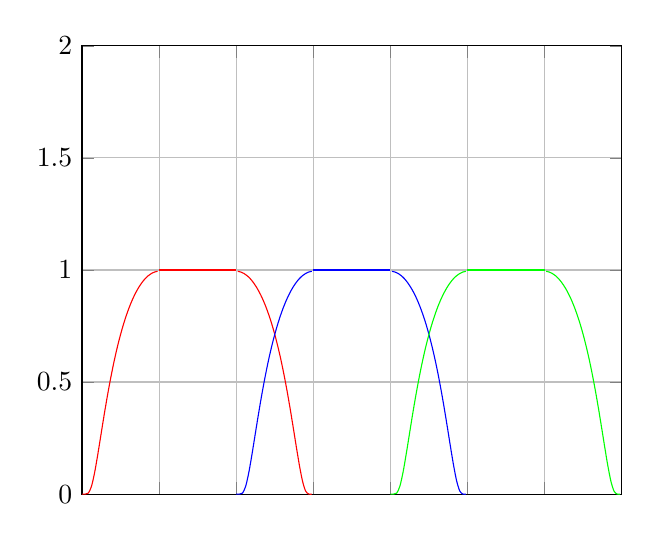
\begin{tikzpicture}
			\begin{axis}[xmin=-1.5,xmax=2,ymin=0,ymax=2,grid=both,xticklabels={}]
				\addplot[domain=-1:-0.5, smooth, red] {1};
				\addplot[domain=-1.5:-1.01, smooth, red] {e^(-(1/4)/((1/4)-(x+1)^2))/0.37};
				\addplot[domain=-0.49:-0.01, smooth, red] {e^(-(1/4)/((1/4)-(x+1/2)^2))/0.37};
				\addplot[domain=0:0.5, smooth, blue] {1};
				\addplot[domain=-0.5:-0.01, smooth, blue] {e^(-(1/4)/((1/4)-(x)^2))/0.37};
				\addplot[domain=0.51:0.99, smooth, blue] {e^(-(1/4)/((1/4)-(x-1/2)^2))/0.37};
				\addplot[domain=1:1.5, smooth, green] {1};
				\addplot[domain=0.5:0.99, smooth, green] {e^(-(1/4)/((1/4)-(x-1)^2))/0.37};
				\addplot[domain=1.51:1.99, smooth, green] {e^(-(1/4)/((1/4)-(x-3/2)^2))/0.37};
			\end{axis}
		\end{tikzpicture}}
	\end{enumerate}
	\end{multicols}
\end{prf}
